\subsubsection*{High inertial effects }
We now turn our attention to the high inertial regime ($Ga =100$).
In this situation it is expected that the presence of wake change completely the flow behavior. 
\begin{figure}[h!]
    \centering
    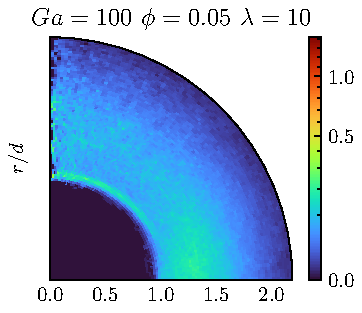
\includegraphics[height=0.21\textwidth]{image/HOMOGENEOUS_NEW/Dist/Pnst_l_10_Ga_100_PHI_0_05.pdf}
    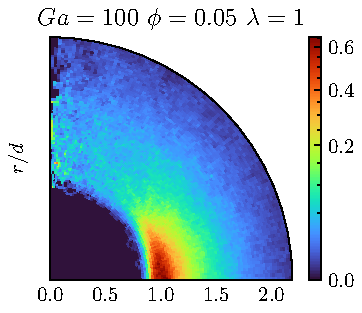
\includegraphics[height=0.21\textwidth]{image/HOMOGENEOUS_NEW/Dist/Pnst_l_1_Ga_100_PHI_0_05.pdf}
    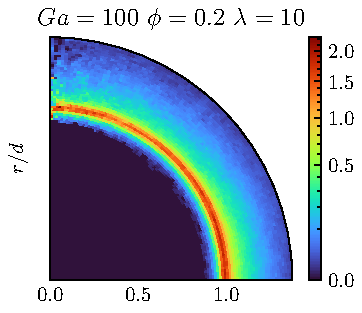
\includegraphics[height=0.21\textwidth]{image/HOMOGENEOUS_NEW/Dist/Pnst_l_10_Ga_100_PHI_0_2.pdf}
    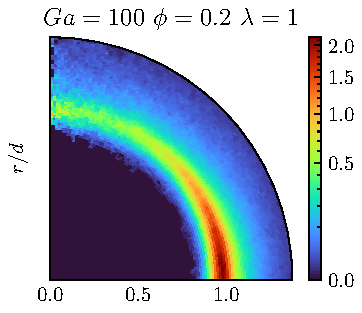
\includegraphics[height=0.21\textwidth]{image/HOMOGENEOUS_NEW/Dist/Pnst_l_1_Ga_100_PHI_0_2.pdf}
    \caption{Histogram of the probability density function $P_\text{nst}$ at high inertial effect $Ga = 100$.
    (left) Low volume fraction cases $\phi=0.05$ for $\lambda = 1,10$.
    (right) High volume fraction cases $\phi=0.1$ for $\lambda = 1,10$ }
    \label{fig:Pnst_high_Ga}
\end{figure}
If we compare \ref{fig:Pnst_high_Ga} (right) with their counterparts from \ref{fig:Pnst_low_Ga} (right) we observe that $P^n_\text{nst}$ becomes even more concentrated at contact of the particles for $Ga=100$.
This could witness of the presence of paced region of particles or clusters. 
In general, all $P_\text{nst}^n$ with $Ga = 100$ exhibit differences compared to the cases with $Ga = 10$. 
Particularly striking, is the presence of anisotropy in the former cases, where a higher concentration of particles is identified at $\theta \approx 0$, as seen in \ref{fig:Pnst_high_Ga}.
Within the high inertial cases, we can notice that $P_\text{nst}^n$ is even more concentrated on the sides for the iso-viscous emulsions ($\lambda = 1$). 
In short, it is clear that the concentration on the side of $P_\text{nst}^n$ increase for increasing $Ga$ and for low viscosity ratio. 
Regarding the volume fraction dependence, it is unclear at this stage if it does or not reduce the presence of such anisotropy.
However, at this stage it remains unclear if increasing $\phi$ have a positive or negative impact on the anisotropy of the distribution. 

To illustrate the impact of $\lambda$ on the microstructure, \ref{fig:images} displays snapshots of two DNS at $\phi = 0.05$ and $Ga = 100$. 
As predicted by $P_\text{nst}^n$, we observe strong layers and particles in close contact for $\lambda = 1$, contrasting with the seemingly more evenly dispersed microstructure for $\lambda = 10$.
\begin{figure}[h!]
    \centering
    % 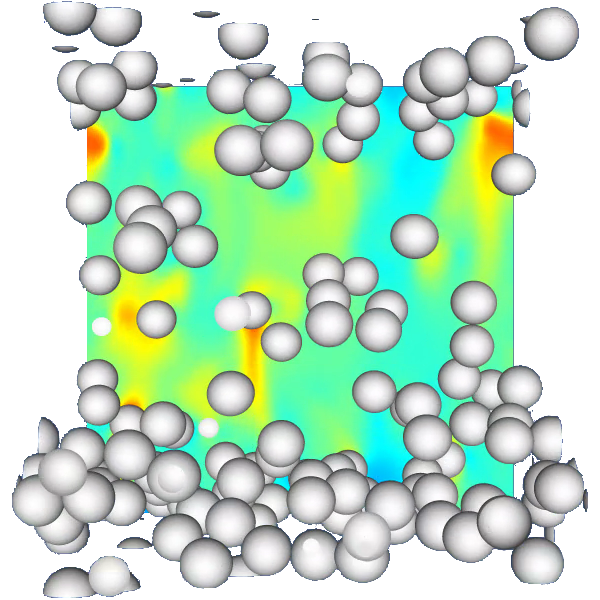
\includegraphics[width=0.3\textwidth]{image/HOMOGENEOUS_NEW/P_PHI_5_l_01_Ga_100.png}
    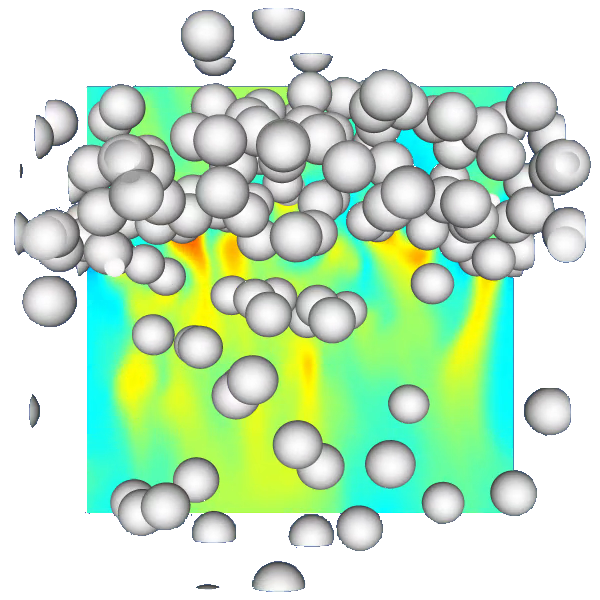
\includegraphics[width=0.4\textwidth]{image/HOMOGENEOUS_NEW/P_PHI_5_l_10_Ga_100.png}
    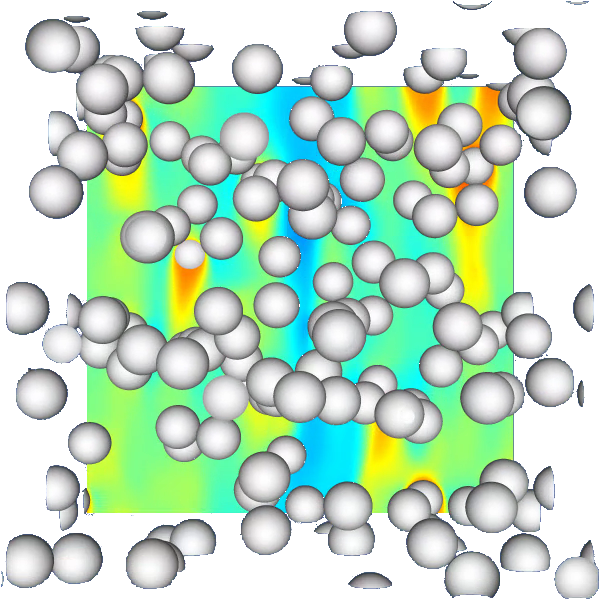
\includegraphics[width=0.4\textwidth]{image/HOMOGENEOUS_NEW/P_PHI_5_l_1_Ga_100.png}
    \caption{Snapshot of a simulation at $t^* = 150$ for $\phi=0.05$ and $Ga=100$.
    Color map : values of the vertical component of the velocity, field on the vertical plane defined by the equation $z=0$. 
    (left)  $\lambda = 1$.
    (right)  $\lambda = 10$.
    }
    \label{fig:images}
\end{figure}
In fact in \ref{fig:images} (right) we can observe horizontal raft of droplets or droplets rising side-by-side, but this effect is clearly not as pronounce as for $\lambda = 1$. 
Clearly, high viscosity ratio appears to maintain a significant distance between particles, which prevent the creation of structures such as droplets layers.
This might be because of a higher vorticity around the viscous droplets.   
% As discussed in \citet{zhang2021three}, rising pairs of spherical bubbles may reach a stable side-by-side configuration, which tends to generate horizontal clusters.
% They range of dimensionless parameters is consistent with the ones presented in this study, making this hypothesis valuable. 
In \citet{legendre2003hydrodynamic} they study the interaction between a pair of bubbles rising side-by-side. 
They stipulate that for two bubbles at moderate Reynolds number $50-100$, the interaction forces is found to be repulsive, while it is attractive or null for higher Reynolds. 
In our case it is reasonable to think that such pair attraction / repulsion mechanisms might also drive the clustering mechanism for the higher \textit{Galileo} cases at $\lambda = 1$.


On another note, we can observe on \ref{fig:images}(left) that the length between the layers is roughly equal to the length of the numerical domain. 
Indeed, only one layer of droplets is present in the domain. 
Therefore, it is hard to known for sure if the current microstructure is constrained by the size of the numerical domain, or if it is well representative of the real microstructure that we would obtain in an infinite non-periodic domain. 
One might argue that the layers appear due to collective effect constrained by the size of the box, since it is exactly what we observe for small number of bubbles rising in a periodic domain, see \citet{loisy2017}. 
However, we might expect that horizontal layers such as the one observed in \ref{fig:images} (left) still remain for lager boxes since they are more probability the cause of pairwise interactions mechanism as discussed above. 
Therefore, we can be sure that layers appear, but the length between these layers is more likely to be constrained by the size of the numerical domain, despite the consequent number of droplets. 
In all rigor, DNS in a larger domain would be required to evaluate the microstructure dependence on the domain size. 
Nevertheless, due to numerical constrains it has not been performed.  

From the present analysis of $P_\text{nst}$ and the actual microstructure presented in \ref{fig:images} we can infer that the \textit{nearest particle statistics} is able to predict features in the microstructure such as layers and clustering effects. 
Which is notable given that, to the author knowledge, no previous studies ever shown such visual proof, in the context of the nearest neighboring statistics. 


\subsection{Nearest radial distribution function }

Although, \ref{fig:Pnst_high_Ga} and \ref{fig:Pnst_low_Ga} give a good representation of the particle pair azimuthal distribution, it is hard to inspect in details the differences in the radial distribution.
Therefore, in \ref{fig:Pr}  we plotted the radial distribution $P_\text{nst}^n(\textbf{x},t,r)$ averaged on all $\theta$.
We displayed two different viscosity ratios and multiples \textit{Galileo} numbers in terms of the dimensionless distance $(r - d)/d_p$ where $d_p$ is the mean particle distance defined as $d_p = n_p^{-1/3}$.  
For a random isotropic distribution of hard spheres it is possible to derive a theoretical prediction for $P_\text{nst}^n(\textbf{x},t,r)$ obtained in the vanishing volume fraction limit. 
Indeed, it is shown in \citet{zhang2021ensemble} that for a dilute random arrangement of particle the probability density of the nearest PDF reads as, 
\begin{equation}
    P_\text{nst}^\text{th}(\textbf{x},t,r) = \exp[{-4 \pi n_p(\textbf{x},t) (r^3 - d^3)/3}].
    \label{eq:Pnst_dilute}
\end{equation}
It must be understood that this formula is accurate only at $\mathcal{O}(\phi)$ therefore in most of our cases it is not expected to be representative. 
Additionally, the hard sphere model differ considerably form the droplets pair distribution since in the latter case $P_\text{nst}^\text{th} = 0$ for $r<d$ while in our case particles might inter-penetrate. 
However, it remains valuable to utilize this theoretical probability density function for comparative purposes. 

\begin{figure}[h!]
    \centering
    % 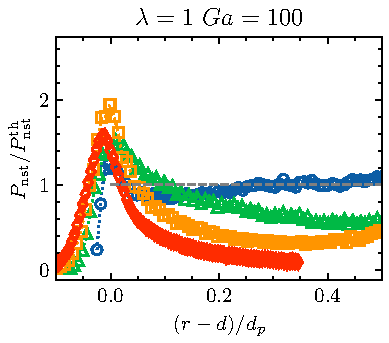
\includegraphics[height=0.3\textwidth]{image/HOMOGENEOUS_NEW/Dist/Pr_l_1_Ga_100.pdf}
    % 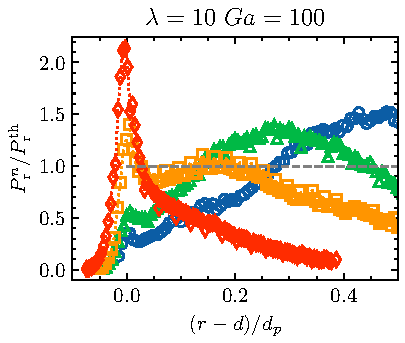
\includegraphics[height=0.3\textwidth]{image/HOMOGENEOUS_NEW/Dist/Pr_l_10_Ga_100.pdf}
    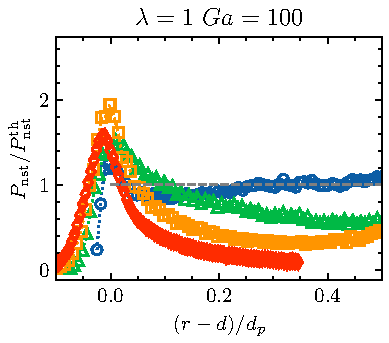
\includegraphics[height=0.3\textwidth]{image/HOMOGENEOUS_NEW/Dist/Pr_l_1_Ga_100.pdf}
    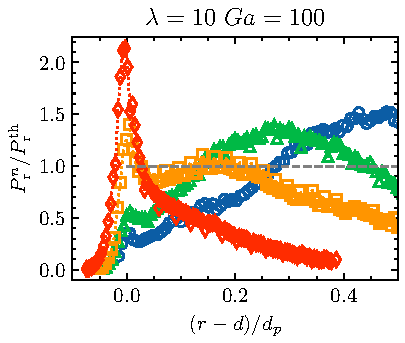
\includegraphics[height=0.3\textwidth]{image/HOMOGENEOUS_NEW/Dist/Pr_l_10_Ga_100.pdf}
    \caption{Radial probability density function $P_\text{nst}^n(\textbf{x},t,r)$ divided by the theoretical distribution \ref{eq:Pnst_dilute}, in terms of the dimensionless distance $(r-d)/d_p$ where, $d_p = n_p^{-1/3}$, for  $Ga = 100$.
    (left)  $\lambda = 1$.
    (right) $\lambda = 10$.
    ($\pmb\bigcirc$) $\phi = 0.01$; ($\pmb\triangle$) $ \phi = 0.05$; ($\pmb\square$) $\phi = 0.1$ ($\pmb\lozenge$) $\phi = 0.2$.
    (dashed lines) Theoretical prediction : $P_\text{nst}^n/P_\text{nst}^\text{th} = 1$. 
    For $r<d$ we arbitrarily set $P_\text{nst}^\text{th} = 1$ so that the distribution can be visualized.
    }
    \label{fig:Pr}
\end{figure}
Surprisingly, In the dilute regime $\phi = 0.01$, we can observe on \ref{fig:Pr} (left) that the radial distribution follow the dilute random arrangement of particle predicted by the theory (\ref{eq:Pnst_dilute}). 
Where for the $\lambda = 10$ at same $\phi$, we notice that the particles are in average further apart from each other. 
In general, for all $\phi$ we observe that the distribution more concentrated at the contact of the particle of reference $(r-d)/d_p = 0$, for $\lambda = 1$ than $\lambda = 10$. 
Although, we selected a small \textit{Bond} number ($Bo = 0.2$), it is clear from \ref{fig:Pr} that the particles inter penetrate with each other as witnessed by the non-vanishing value of $P_\text{nst}$ for $r-d<0$.

In short, we observed that both, the radial and azimuthal distribution were affected by the inertial effect measured by the \textit{Galileo} number. 
The major effect coming with high inertia is the generation of strong anisotropy in the particle pair distribution, as well as a more important concentration of neighboring particles at close contact of the particles of reference. 
Regarding the viscosity ratio, it has a strong impact on the emulsion distribution  only at high $Ga$, whereas at low $Ga$ the change in viscosity ratio has no notable impact on $P_\text{nst}$, as seen in \ref{fig:Pnst_low_Ga}. 


\subsection{Macroscopic modeling of the microstructure}
Up to now, we have presented visualizations of the microstructure with 2D or 1D distributions. 
However, for a more quantitative description, we would like to adopt a different approach. 
Following \citet{zhang2023evolution}, we opt to describe the microstructure using the second moment of $P_\text{nst}$ with respect to \textbf{r}, it reads,
\begin{equation}
    \textbf{R}(\textbf{x},t) =\frac{1}{n_p(\textbf{x},t)} 
    \int_0^\infty 
    \int_{\mathbb{R}^3} \textbf{rr} P_\text{nst}(\textbf{x},\textbf{r},t,a) d\textbf{r} da.
    \label{eq:R}
\end{equation}
This second-rank tensor measures the spread of the nearest neighbor distribution in a given direction. 
It's worth noting that such a quantity is computable only because $\lim_{|\textbf{r}|\to \infty} P(\textbf{x},\textbf{r},t,a) = 0$, which enables the integral of \ref{eq:R} to converge. 
This wouldn't be the case for classic pair distributions, which is the primary reason why we use the \textit{nearest particle statistic} framework. 

Since our objective is to measure the anisotropy of the microstructure, we are particularly interested in the deviatoric part of this tensor, namely,
\begin{equation*}
    \textbf{A}(\textbf{x},t) = \textbf{R}(\textbf{x},t) - \frac{1}{3} [\textbf{R}(\textbf{x},t) : \textbf{I}] \textbf{I}.
\end{equation*}
The tensor $\textbf{R}(\textbf{x},t)$ permits us to measure the mean square distance between a particle and its nearest neighbor, in average and in the three dimension of space. 
Therefore, $\textbf{A}(\textbf{x},t)$ represents likelihood of having a particle in a given direction. 
Thus, for an isotropic suspension $A_{xx} = A_{xx} = 0$. 
In a scenario such as the one depicted in \ref{fig:images} (left), it's evident that $A_{yy} < 0 < A_{xx} \approx A_{zz}$, as a particle is more likely to have its nearest neighbor on the sides rather than on the verticals.
For a better interpretation of the following results it is of interest to compute the distance $r_m$, which is the mean distance to the nearest neighboring particle in a random distribution of hard sphere. 
By direct integration of \ref{eq:Pnst_dilute} we find, 
\begin{equation*}
    r_m^2 /d^2
    = \textbf{I}:\textbf{R}(\textbf{x},t)/d^2
    = {{4^{{{2}\over{3}}}\,\Gamma\left({{5}\over{3}} , 8\,\phi\right)
    \,e^{8\,\phi}}\over{2^{{{10}\over{3}}}\,\phi^{{{2}\over{3}}}}}
\end{equation*}
where $\Gamma(z,a) = \int_a^\infty t^{z-1} e^{-t} dt$ is the upper incomplete gamma function. 

\begin{figure}[h!]
    \centering
    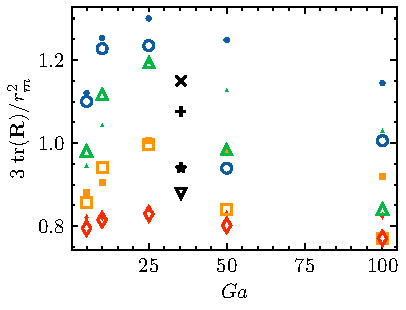
\includegraphics[height=0.3\textwidth]{image/HOMOGENEOUS_NEW/PA/trR.pdf}
    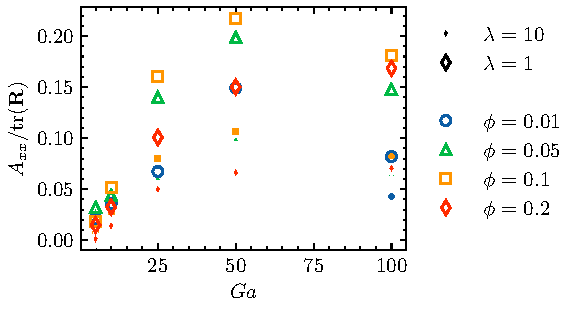
\includegraphics[height=0.3\textwidth]{image/HOMOGENEOUS_NEW/PA/Axx.pdf}
    \caption{
        (left) Trace of the second moment of the probability density function $P_\text{nst}(\textbf{r})$ divided by the square diameter of the particles $d^2$. 
        (right) vertical components of the anisotropy tensor divided by the trace of the second moment of the probability density function.
    ($\pmb\bigcirc$) $\phi = 0.01$; ($\pmb\triangle$) $ \phi = 0.05$; ($\pmb\square$) $\phi = 0.1$ ($\pmb\lozenge$) $\phi = 0.2$.
    The hollow symbols correspond to $\lambda = 1$, the filled symbols to $\lambda = 10$.
    For $r<d$ we arbitrarily set $P_\text{nst}^\text{th} = 1$ so that the distribution can be visualized.
    Black symbols represent the results of \citet{zhang2023evolution} for hard sphere suspension with $\phi = 0.016,0.056,0.134,0.262$  %$\phi = 0.0168,0.0565,0.1341,0.2622$ 
    corresponding to $\pmb\times,\pmb +, \pmb\star , \pmb\triangledown$, respectively.
    }
    \label{fig:A}
\end{figure}
\ref{fig:A} (left) displays the value of the mean square distance : $\textbf{I}:\textbf{R}/r_m^2$, between nearest neighbors for all our numerical cases. 
To help comprehension, first notice that the simulation denoted by the symbol \textcolor{col1}{$\pmb\circ$} in \ref{fig:A} (left), corresponding to $\lambda = 1$, $Ga = 100$ and $\phi = 0.01$, has a value of $\textbf{I}:\textbf{R}/r_m^2 = 1$. Which is consistent with the quasi hard sphere distribution reported for this case in \ref{fig:Pr} (left). 
It is clear from the graph that the mean square distance is mainly dependent on the volume fraction. 
We observe that $\textbf{I}:\textbf{R}/r_m^2$  decrease for increasing $\phi$, which means that particles get in average closer to one another compared to a hard sphere random distribution. 
As noted by \citet{zhang2023evolution} this implies the apparition of clusters as the particles get packed. 
The dependence on the \textit{Galileo} number is non-monotonic, indeed, $\textbf{I}:\textbf{R}/r_m^2$ the distance is increasing until $Ga = 25$ and the decreasing until $Ga = 100$.  
At rather high $Ga$ one might notice that the mean square distance for $\lambda = 1$ (hollow symbols) is lower. 
For all our DNS we observe that the distance to the nearest neighbor for iso-viscous emulsions is on average more distant for $\lambda = 10$ which is consistent with the distributions displayed \ref{fig:Pr} and the picture from \ref{fig:images}.  
On \ref{fig:A} (left) the symbols : $\pmb\star, \pmb\times,\pmb +, \pmb\triangledown$, represent the results of \citet{zhang2023evolution} for hard sphere sedimentation. 
As observed, the value of $\textbf{R}:\textbf{I}$ is on average closer to $r_m^2$ than our simulations, but it maintains the same trend, i.e., clusters appear as the volume fraction increases.
 
Regarding the anisotropy measure we can see on \ref{fig:A} (right) that we have $A_{xx} \ge 0$ for nearly all our cases, meaning that globally, the emulsion is either isotropic ($A_{xx} = 0$), or with particles that are in average more aligned horizontally ($A_{xx} >0$). 
Then, we can see that $A_{xx}$ increase until $Ga = 50$ where we reach the maximum $A_{xx}$, and then decrease until $Ga =100$  but still remains consequent. 
Consistently with the cases from \ref{fig:images} where the value of $A_{xx}$ is greater for $\lambda = 1$ lower for  $\lambda = 10$.
Although, it is not quite obvious we observe a non-monotonic trends with the volume fraction, $A_{xx}$ first increase up to a maximum value for $\phi =0.1$ (represented by \textcolor{col3}{$\pmb\square$} on \ref{fig:A} (right)) and then decrease for $\phi=0.2$ (represented by the \textcolor{col4}{$\pmb\lozenge$} symbols). 
This implies that at a certain volume fraction, around $\phi \approx 0.1$, higher volume fractions tend to randomize the emulsion, while at moderate volume fractions, it favors the side-by-side configuration.
This phenomenon of isotropisation at high $\phi$ has been reported in other studies such as in \citet{seyed2021sedimentation} for sedimentation of solid particles. 
However, at high \textit{Galileo} number it seems that this effect is less pronounced. 
In short, we observed that the mean square particle distance compared to a random case were decreasing with the volume fraction, and is higher for viscous particles ($\lambda = 10$) at high $Ga$, meanwhile the likelihood of finding a nearest neighboring particle on the horizontal is greater for $\lambda=1$ than $\lambda = 10$, and it is globally increasing with higher $Ga$ and non-monotonic with $\phi$. 


\paragraph*{Bibliography : } 
Although, previous studies mainly focused on bubbles or solid particles, it is reasonable to compare the $\lambda = 1$ and $\lambda = 10$ DNS, to the former and the latter cases, respectively. 
In \citet{bunner2002dynamics} they performed tri-periodic simulation of buoyant bubbles at $Re \approx 10-30$ depending on $\phi$.
They reported a preference for the bubbles to be aligned in pair. 
Which is consistent with what we observe in \ref{fig:A} (right) since the anisotropy tensor $A_{xx}$ is clearly positive for $Ga = 25$ (which correspond roughly to $Re = 25$) for $\lambda = 1$ cases (represented by hollow symbols). 
Here we argue that for low viscosity ratio $\lambda = 1$ and $Ga = 100$ we recover potential flow limit interactions which makes the side-by-side configuration more stable \citep{legendre2003hydrodynamic}, so that even more side-by-side configuration are observed. 

For solid particles at $Ga = 144$ it is observed in \citet{shajahan2023inertial} that in the dilute regime, $\phi \approx 0.02$, verticals raft of particles are formed. 
In our case we could not observe such a phenomenon, meaning that it might arise at even higher viscosity ratio or \textit{Galileo} number. 
The latter effect is explained by the presence of a more developed wake for dilute solid particles which trap neighboring particles within the wake without repulsing it on the sides. 
In our case we observe more particles in the verticals' directions for $\lambda = 10$ than $\lambda =1$ at $Ga =100$ in \ref{fig:A}(right), since $A_{xx}$ is smaller in the former cases.
Although it is not quite obvious it might be the consequence of the same effects, i.e., the wake of the viscous drop might induce less side-by-side configuration and more vertical nearly stable configuration. 
DNS at higher $Ga$ and $\lambda$ would be necessary to confirm or not the presence of the wake trapping effect.  
In the moderately dense regime,  $0.02 < \phi \le 10$ they identified more configuration of particles situated side-by-side. 
As mentioned above even if it is less pronounce than for the iso-viscous case we indeed observe that on \ref{fig:A} (right) for $\lambda = 10$. 


Ultimately, \ref{fig:A} constitutes a significant result of this work as it quantifies the microstructure using only the second rank tensor $\textbf{R}(\textbf{x},t)$.
For future perspectives, based on the value of $\textbf{R}(\textbf{x},t)$, an approximation of the distribution could be reconstructed by assuming a certain functional form with 2 degrees of freedom, corresponding to the scalars $\textbf{R}:\textbf{I}$ and $A_{xx}$.
This approximated distribution could then be used to better solve certain theoretical problems involving the theoretical pair distribution function (\citet{batchelor1972sedimentation}, \citet{hinch1977averaged}, and \citet{zhang2021ensemble}).
In the following we try to explain the origin of the striking difference between $\lambda = 1$ and $\lambda = 10$ on the particle pair distribution.
With this objective in mind, we present a meticulous analysis of the particle time of interaction as well as the particles relative averaged velocity fields. 
